\documentclass[12pt]{article}%
\usepackage{amsfonts}
\usepackage{fancyhdr}
\usepackage{comment}
\usepackage[a4paper, top=2.5cm, bottom=2.5cm, left=2.2cm, right=2.2cm]%
{geometry}
\usepackage{pdfpages}
\usepackage{times}
\usepackage{amsmath}
\usepackage{changepage}
\usepackage{amssymb}
\usepackage{graphicx}%
\setcounter{MaxMatrixCols}{30}
\newtheorem{theorem}{Theorem}
\newtheorem{acknowledgement}[theorem]{Acknowledgement}
\newtheorem{algorithm}[theorem]{Algorithm}
\newtheorem{axiom}{Axiom}
\newtheorem{case}[theorem]{Case}
\newtheorem{claim}[theorem]{Claim}
\newtheorem{conclusion}[theorem]{Conclusion}
\newtheorem{condition}[theorem]{Condition}
\newtheorem{conjecture}[theorem]{Conjecture}
\newtheorem{corollary}[theorem]{Corollary}
\newtheorem{criterion}[theorem]{Criterion}
\newtheorem{definition}[theorem]{Definition}
\newtheorem{example}[theorem]{Example}
\newtheorem{exercise}[theorem]{Exercise}
\newtheorem{lemma}[theorem]{Lemma}
\newtheorem{notation}[theorem]{Notation}
\newtheorem{problem}[theorem]{Problem}
\newtheorem{proposition}[theorem]{Proposition}
\newtheorem{remark}[theorem]{Remark}
\newtheorem{solution}[theorem]{Solution}
\newtheorem{summary}[theorem]{Summary}
\newenvironment{proof}[1][Proof]{\textbf{#1.} }{\ \rule{0.5em}{0.5em}}

\newcommand{\Q}{\mathbb{Q}}
\newcommand{\R}{\mathbb{R}}
\newcommand{\C}{\mathbb{C}}
\newcommand{\Z}{\mathbb{Z}}

\begin{document}

    \title{CS280 Spring 2023 Assignment 2 \\ Part A}
    \author{Convolutional Neural Network}
    \maketitle

    \paragraph{Name: Bingnan Li}

    \paragraph{Student ID: 2020533092}

    \newpage


    \subsubsection*{1. Convolution Cost (10 points)}
    Assume an input of shape  $c_i\times h\times w$  and a convolution kernel of shape  $c_o\times c_i\times k_h\times k_w$ , padding of  $(p_h,p_w)$ , and stride of  $(s_h,s_w)$ .
    \begin{itemize}
        \item What is the computational cost (multiplications and additions) for the forward propagation?\\
        {\bf Solution:}
        \par The output size has the formula as follows:
        \[c_{out}=\#\{kernels\}\]
        \[h_{out}=\left\lfloor\frac{h_{in}+2\times padding\_size_h-(kernel\_size_h-1)-1}{stride\_size_h}+1\right\rfloor \]
        \[w_{out}=\left\lfloor\frac{w_{in}+2\times padding\_size_w-(kernel\_size_w-1)-1}{stride\_size_w}+1\right\rfloor \]
        Substitute $h_{in}, w_{in}, padding\_size_h, padding\_size_w, stride\_size_h, stride\_size_w, kernel\_size_h$ and $kernel\_size_w$
        with $h, w, p_h,p_w,s_h,s_w,k_h$ and $k_w$ respectively, the output size is
        \[c_{out}=c_0\]
        \[h_{out}=\left\lfloor\frac{h+2p_h-k_h}{s_h}+1\right\rfloor \]
        \[w_{out}=\left\lfloor\frac{w+2p_w-k_w}{s_w}+1\right\rfloor \]

        Then for each element in output, it is calculated by $c_i\times k_h\times k_w$ times multiplications and $c_i\times k_h\times k_w - 1$ times additions.
        Thus, the computational cost is
        \[cost = c_0\left\lfloor\frac{h+2p_h-k_h}{s_h}+1\right\rfloor\left\lfloor\frac{w+2p_w-k_w}{s_w}+1\right\rfloor\left(2c_i k_h k_w-1\right)\]
        \item What is the memory footprint?\\
        {\bf Solution:}
        \par Based on the previous analysis, we know the output size is
        \[\left(c_0,\left\lfloor\frac{h+2p_h-k_h}{s_h}+1\right\rfloor,\left\lfloor\frac{w+2p_w-k_w}{s_w}+1\right\rfloor\right)\]
        So the memory footprint of output is
        \[c_0\left\lfloor\frac{h+2p_h-k_h}{s_h}+1\right\rfloor\left\lfloor\frac{w+2p_w-k_w}{s_w}+1\right\rfloor\]
        and the total memory footprint including input and kernels is
        \[c_0\left\lfloor\frac{h+2p_h-k_h}{s_h}+1\right\rfloor\left\lfloor\frac{w+2p_w-k_w}{s_w}+1\right\rfloor + c_i h w+c_0 c_i k_h k_w\]
    \end{itemize}

    \newpage


    \subsubsection*{2. Convolution Kernel (10 points)}
    Assume there are two convolution kernels of size
    $k_1$ and $k_2$ respectively (with no nonlinear activation function in-between).
    \begin{itemize}
        \item Prove that the results of the two convolution operations can be expressed by a single convolution operation.\\
        {\bf Proof:}
        \par Define the input as $X$ and $Y,Z$ are the output of the first and the second convolution layer, where
        \begin{align*}
            Y = conv_1(X)\\
            Z = conv_2(Y)
        \end{align*}
        Then define $A(x,y)$ as the element at position $(x,y)$ of $A$.
        By the definition of convolution operation, we have
        \begin{align*}
            Z(i,j) &= \sum_{p=0}^{k_2-1}\sum_{q=0}^{k_2-1}kernel_2(p,q)Y(i+p,j+q)\\
            Y(i+p,j+q) &= \sum_{m=0}^{k_1-1}\sum_{n=0}^{k_1-1}kernel_1(m,n)X(i+p+m,j+q+n)
        \end{align*}
        Substitute $Y(i+p,j+q)$ into $Z(i,j)$ and we get:
        \begin{align*}
            Z(i,j) &= \sum_{p=0}^{k_2-1}\sum_{q=0}^{k_2-1}kernel_2(p,q)\sum_{m=0}^{k_1-1}\sum_{n=0}^{k_1-1}kernel_1(m,n)X(i+p+m,j+q+n)\\
            &= \sum_{p=0}^{k_2-1}\sum_{q=0}^{k_2-1}\sum_{m=0}^{k_1-1}\sum_{n=0}^{k_1-1}kernel_2(p,q)kernel_1(m,n)X(i+p+m,j+q+n)\\
            &= \sum_{a=0}^{k_3-1}\sum_{b=0}^{k_3-1}kernel_3(a,b)X(i+a,j+b)
        \end{align*}
        where $k_3 = k_2+k_1-1$ and
        \begin{align*}
            kernel_3(a, b) &= \sum_{x=\max(0,a-k_1+1)}^{\min(a,k_2-1)}\sum_{x=\max(0,b-k_1+1)}^{\min(b,k_2-1)}kernel_2(x,y)\cdot kernel_1(a-x,b-y)\\
            &= kernel_2 * kernel_1
        \end{align*}
        {\bf Remark:} $kernel_3$ is the "real" convolution result between $kernel_1$ and $kernel_2$.
        It's different from the image convolution operation described in the question, which is actually correlation operation.
        \par Since $Z(i,j) = \sum_{a=0}^{k_3-1}\sum_{b=0}^{k_3-1}kernel_3(a,b)X(i+a,j+b)$, $Z(i,j)$ can be computed from single convolution.
        \item What is the dimensionality of the equivalent single convolution?\\
        {\bf Solution:}
        \par Based on the previous proof, we know $Z(i,j) = \sum_{a=0}^{k_3-1}\sum_{b=0}^{k_3-1}kernel_3(a,b)X(i+a,j+b)$ where $k_3=k_1+k_2-1$,
        we know that the kernel size of equivalent single convolution is $(k_1+k_2-1)\times (k_1+k_2-1)$.
        \item Is the converse true, i.e.,
        Can a convolution operation be decomposed into two smaller convolution operations?\\
        {\bf Solution:}
        \par The converse is false, because any convolution kernel can be decomposed into two smaller convolution kernels means
        that the elements in the large kernel are constrained to be the sum of partial elements in the small kernels.
        However, this limits the degree of freedom of large kernel.
        For example, if we have two convolution kernels $kernel_1$ and $kernel_2$ with size $3\times 3$ and $5\times 5$ respectively,
        then the kernel $kernel_3$ with size $7\times 7$ can be decomposed into two smaller kernels $kernel_1$ and $kernel_2$ (full-convolution).
        However, the degree of freedom of $kernel_3$ is no longer $7\times 7 = 49$ but $3\times 3+5\times 5 = 34$, so the solution space is much smaller
        and there must be at least one kernel that can not be decomposed into two smaller kernels.
    \end{itemize}

    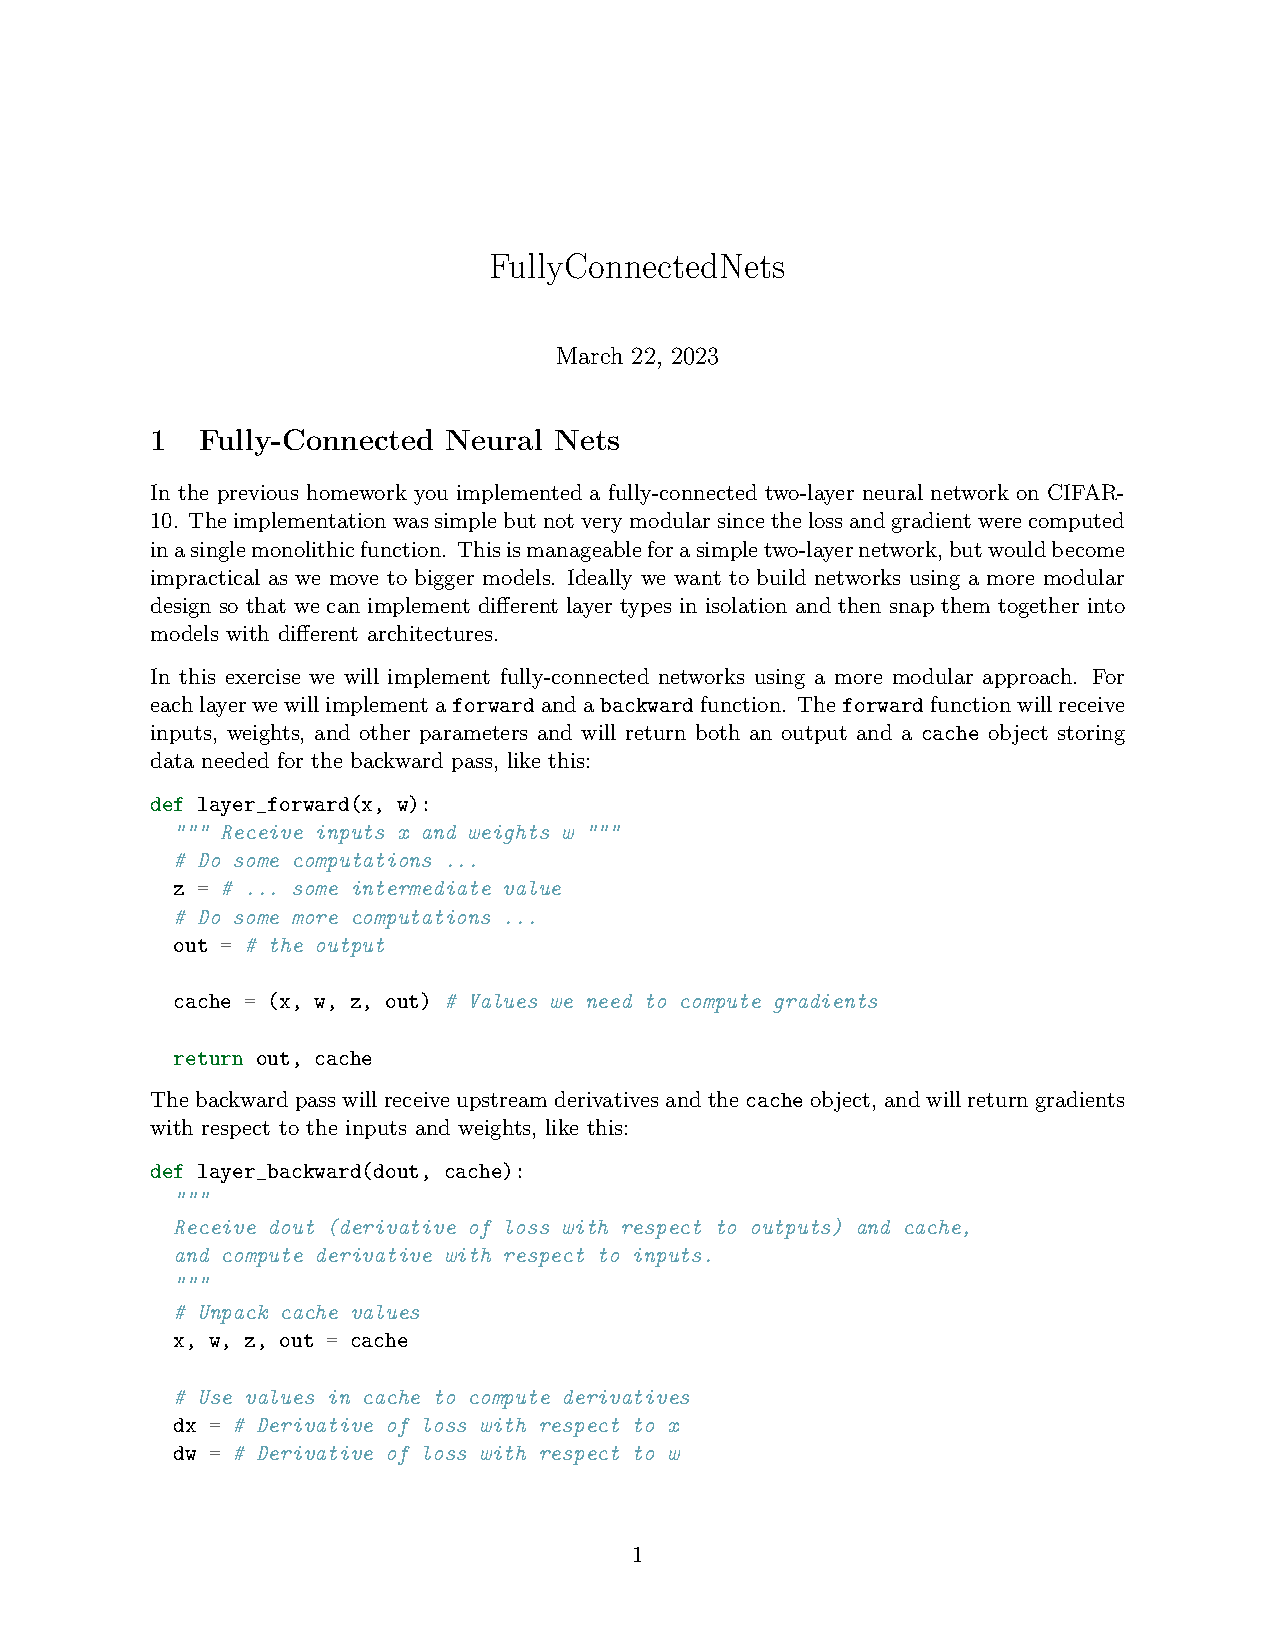
\includepdf[pages=1-]{../out/FullyConnectedNets.pdf}
    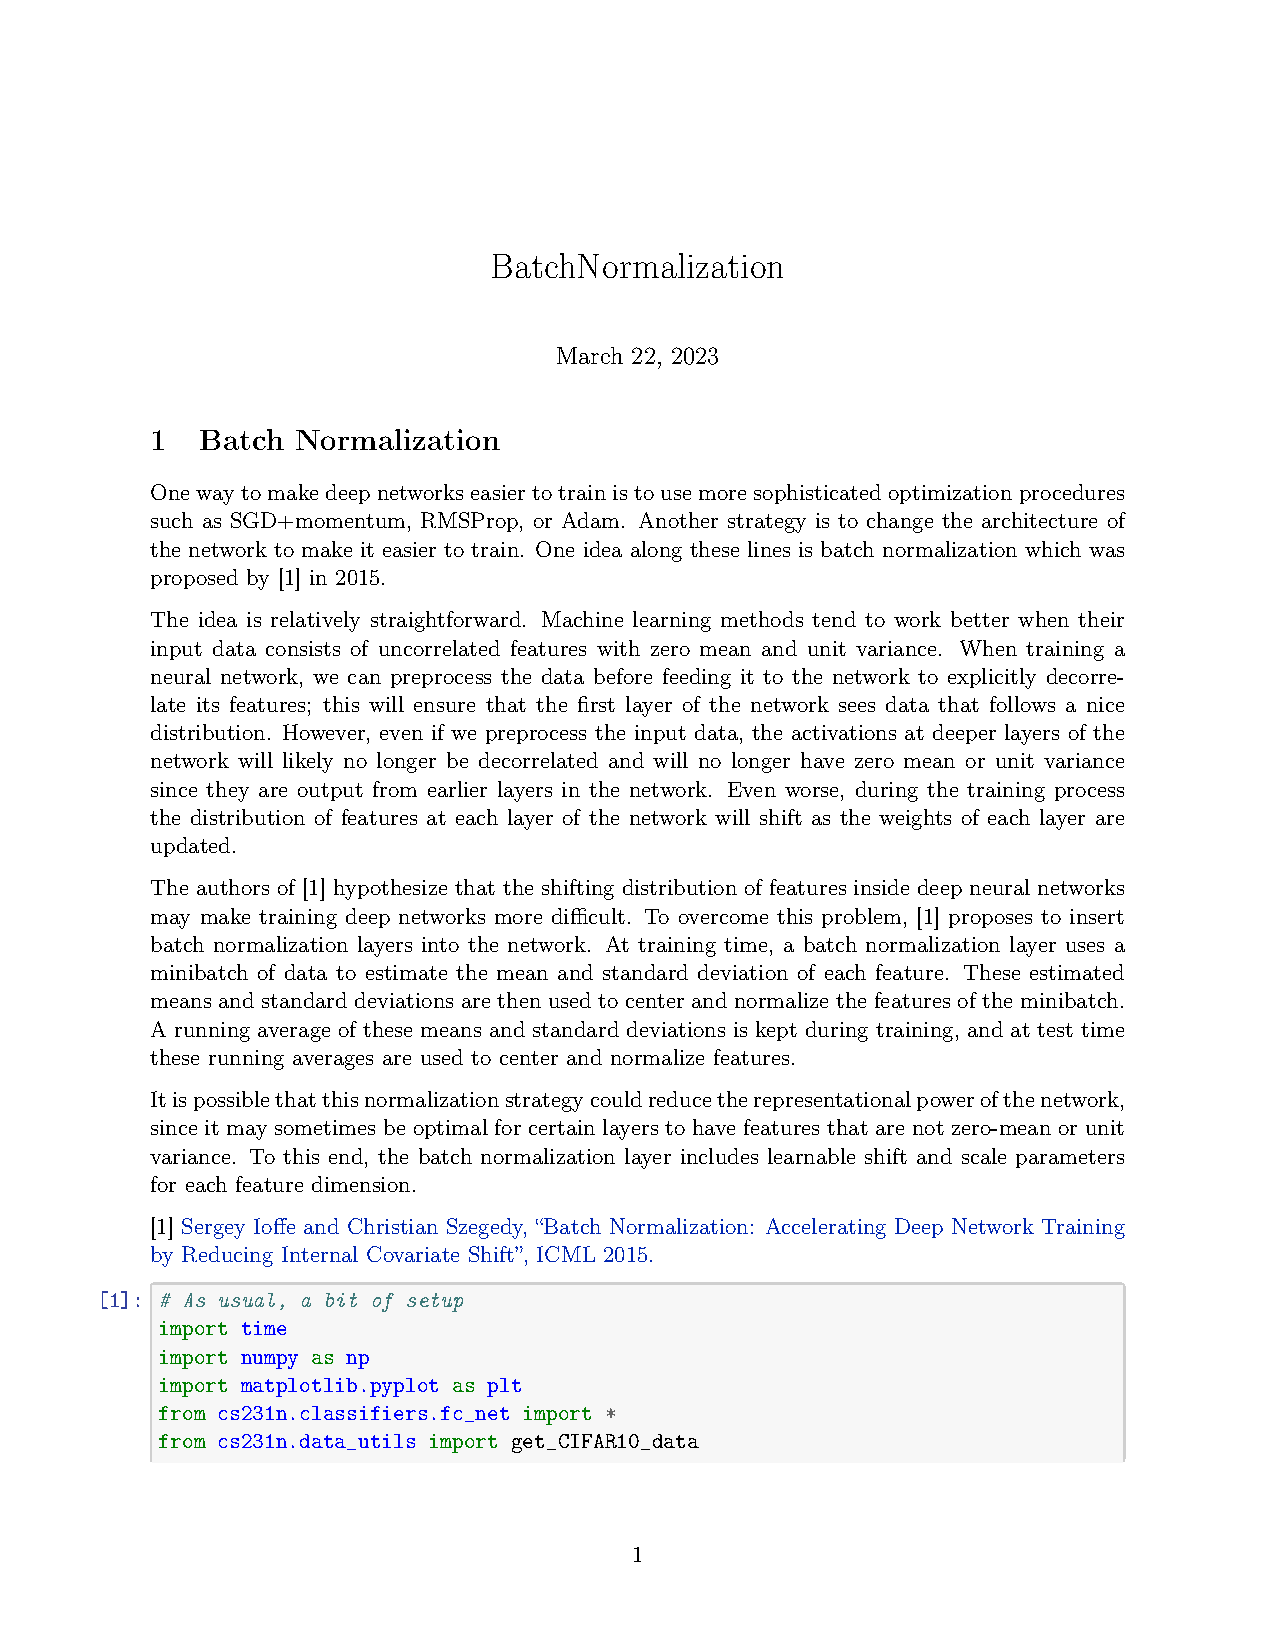
\includepdf[pages=1-]{../out/BatchNormalization.pdf}
    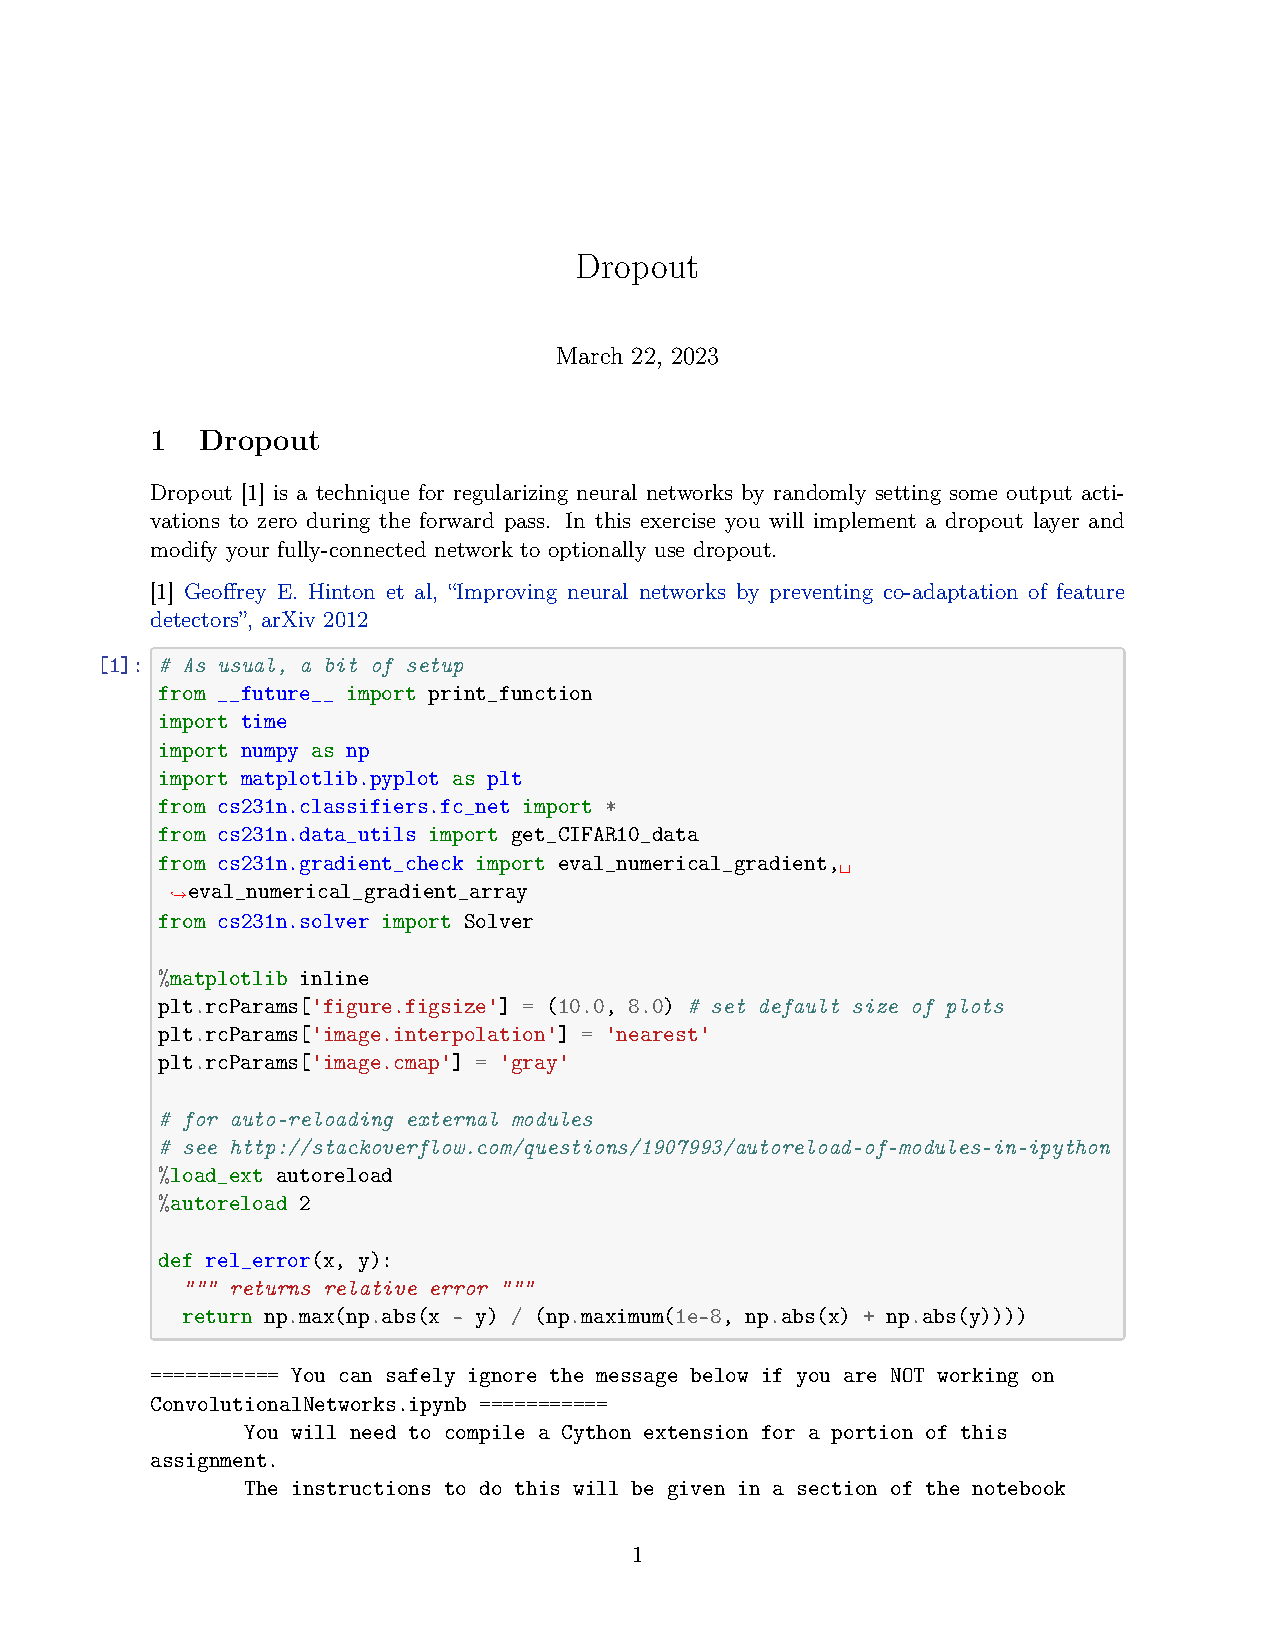
\includepdf[pages=1-]{../out/Dropout.pdf}
    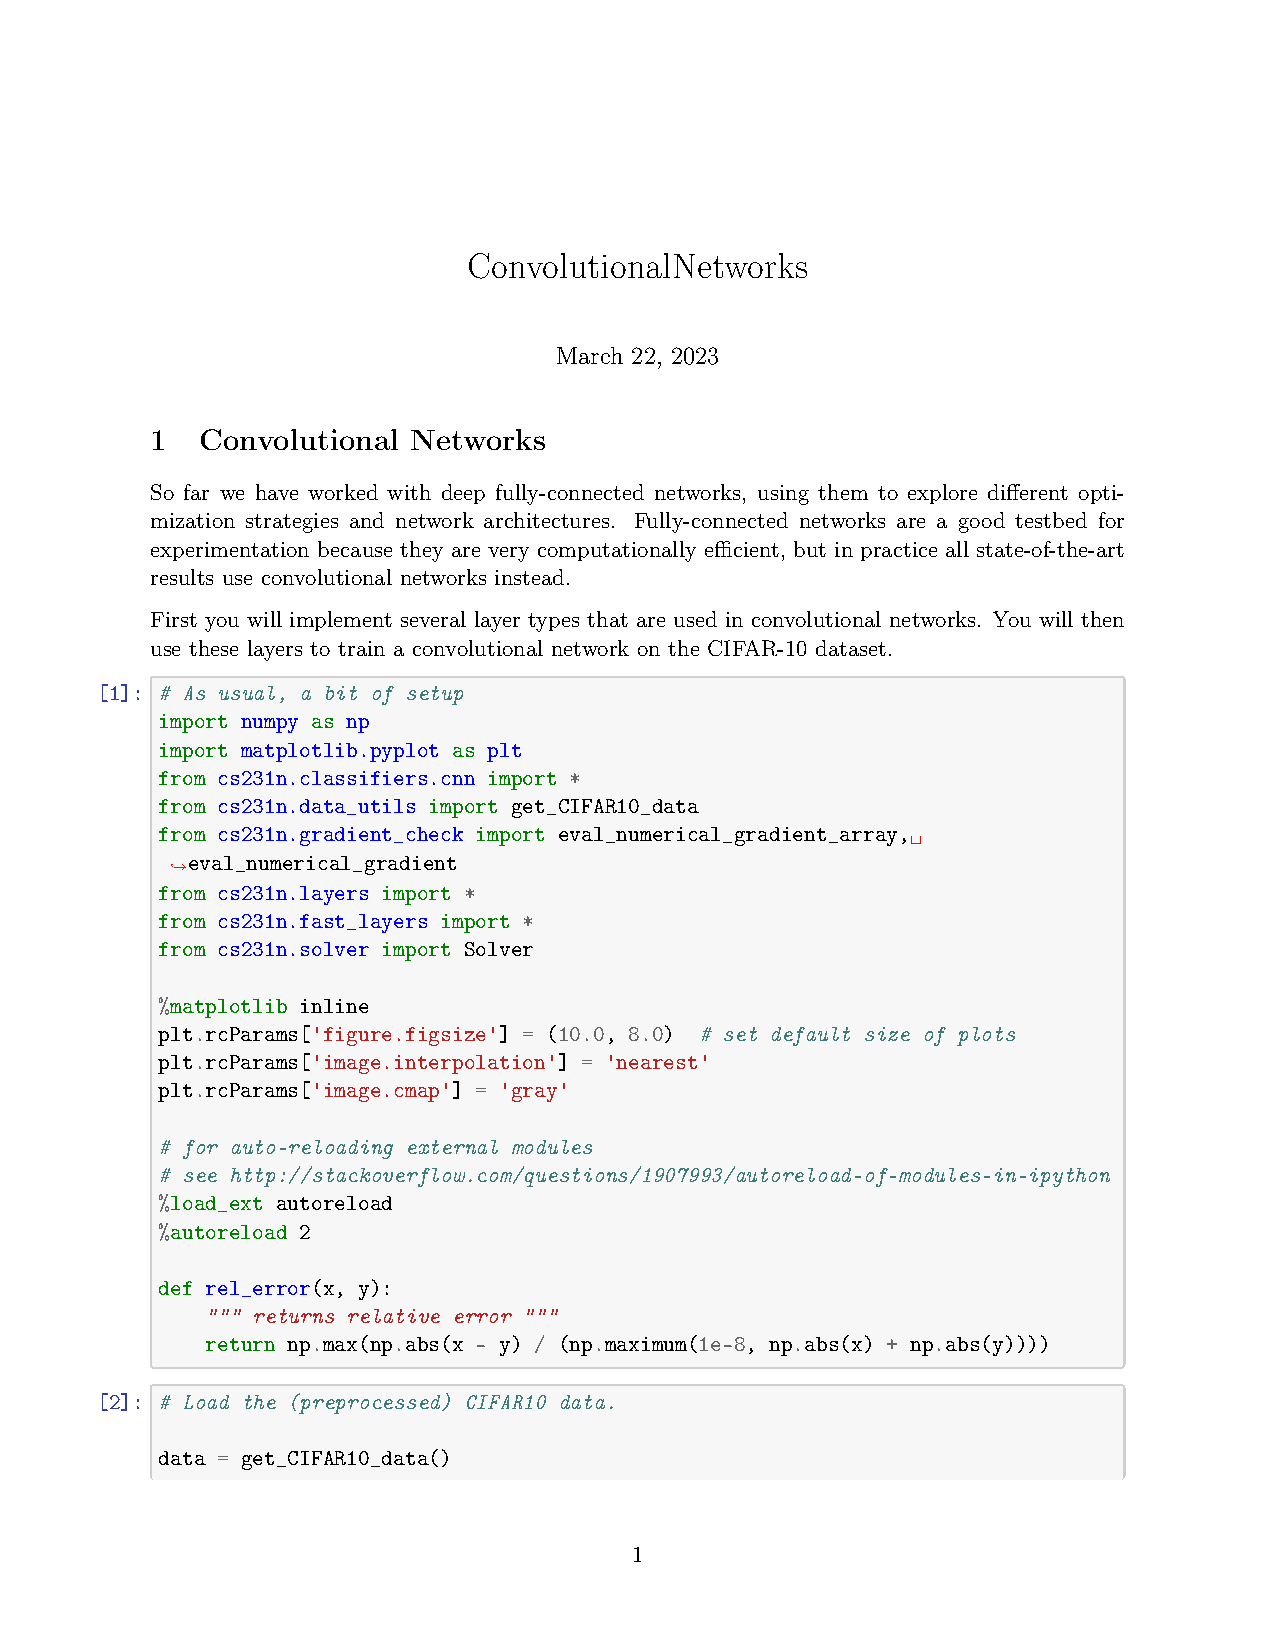
\includepdf[pages=1-]{../out/ConvolutionalNetworks.pdf}
    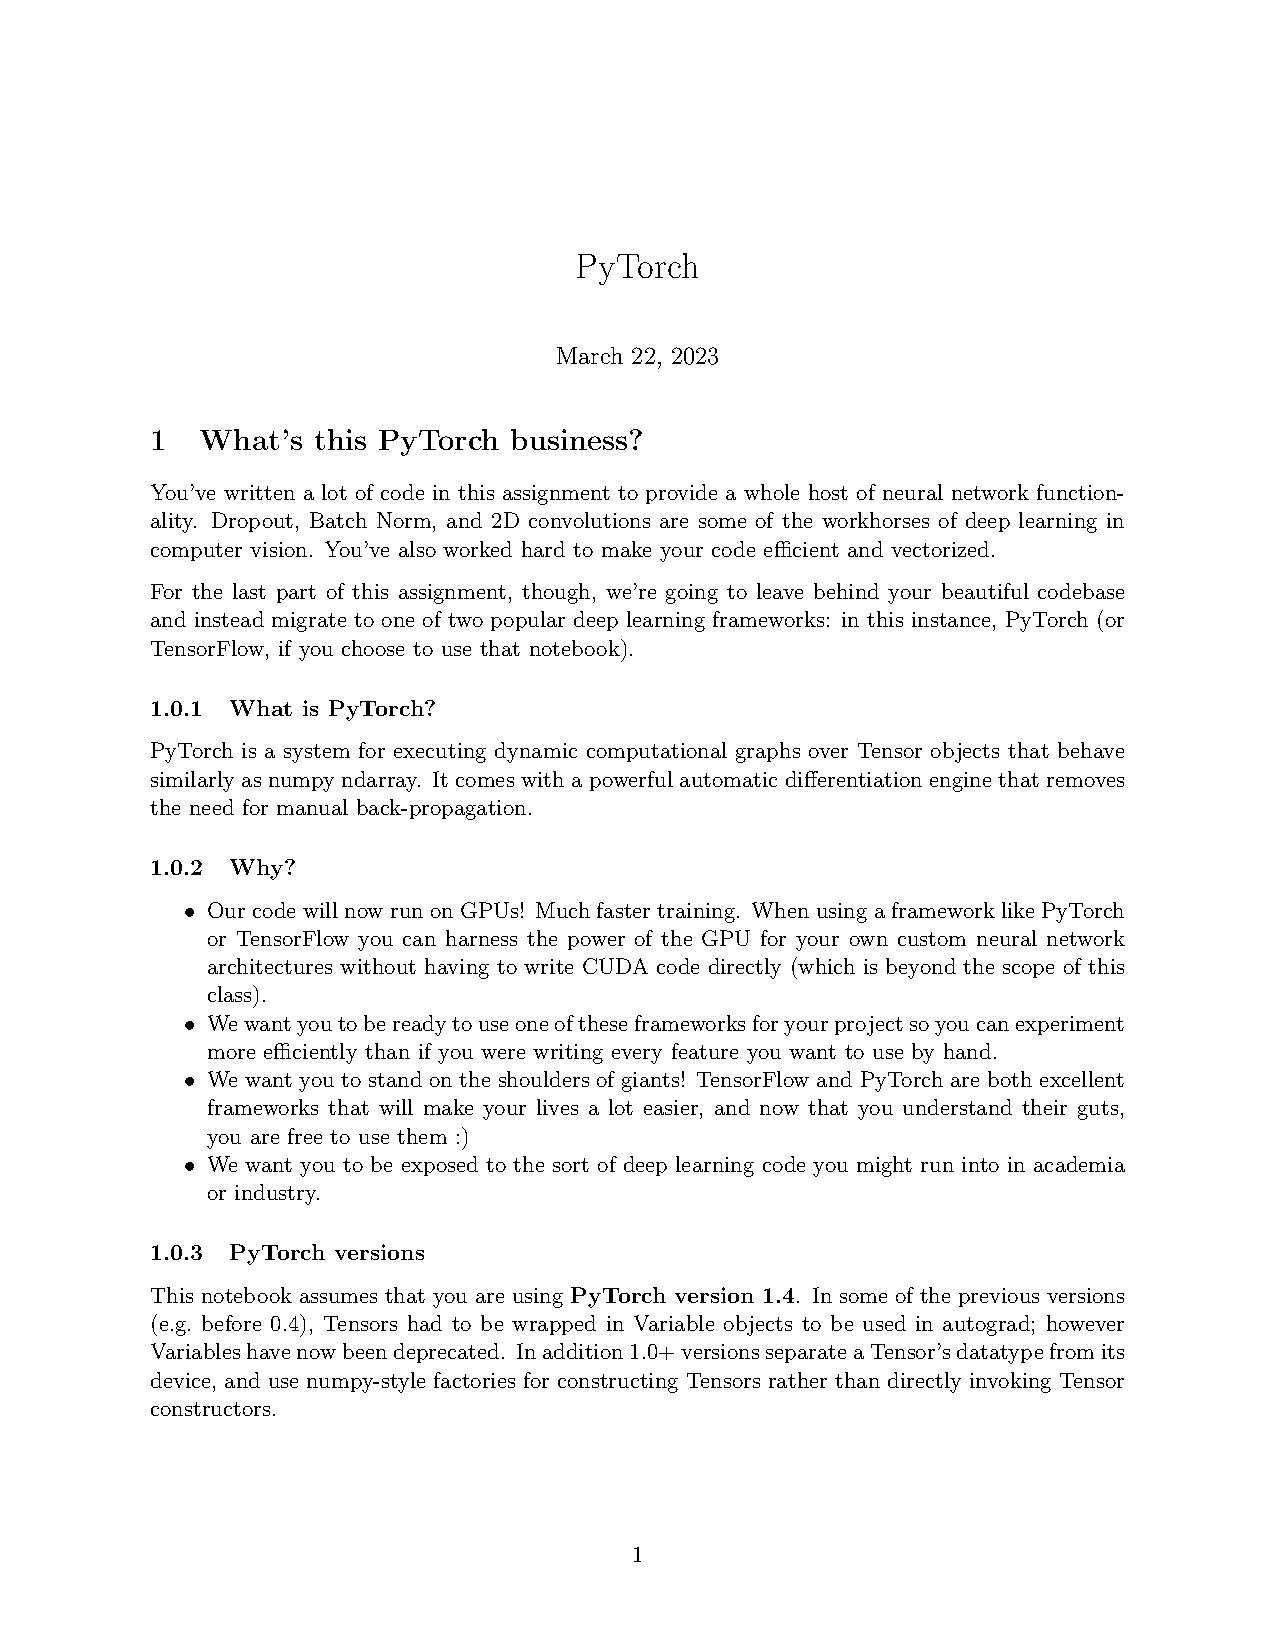
\includepdf[pages=1-]{../out/PyTorch.pdf}
\end{document}